\باب{سمتی تفرقی علم الاحصاء۔ سمتی تفاعل}

\حصہ{غیر سمتی میدان اور سمتی میدان}
غیر سمتی تفاعل سے مراد ایسا تفاعل ہے جو فضا میں کسی سلسلہ نقاط کے ہر نقطے  پر معین ہو اور جہاں تفاعل کی قیمتیں حقیقی اعداد ہوں جن کا دارومدار صرف فضا میں نقطوں پر ہو نا کہ چنی گئی محوری نظام پر۔ان نقطوں کے سلسلے کو تفاعل کا \اصطلاح{دائرہ کار}\فرہنگ{دائرہ کار}\حاشیہب{domain}\فرہنگ{domain} کہتے ہیں۔عملی استعمال میں تفاعل \عددی{f} کا دائرہ کار \عددی{D} عموماً  منحنی یا سطح یا فضا میں تین بُعدی خطہ ہو گا۔تفاعل \عددی{f} دائرہ کار \عددی{D} کے ہر نقطے کے ساتھ ایک غیر سمتی حقیقی عدد وابستہ کرتا ہے اور ہم کہتے ہیں کہ \عددی{D} میں \اصطلاح{غیر سمتی میدان}\فرہنگ{غیر سمتی!میدان}\فرہنگ{میدان!غیر سمتی}\حاشیہب{scalar field}\فرہنگ{scalar!field}\فرہنگ{field!scalar} دیا گیا ہے۔

\عددی{x}، \عددی{y}، \عددی{x} متعارف کرنے سے تفاعل \عددی{f} کو ان محدد کی مدد سے \عددی{f(x,y,z)} لکھا جا سکتا ہے، پس اتنا یاد رہے کہ کسی بھی نقطہ \عددی{P} پر  تفاعل \عددی{f} کی قیمت، چنی گئی محددی نظام پر ہرگز منحصر نہیں ہو گی۔اس حقیقت کو ظاہر کرنے کی خاطر \عددی{f(x,y,z)} کی جگہ عموماً \عددی{f(P)} لکھا جاتا ہے۔تفاعل \عددی{f} وقت پر بھی منحصر ہو سکتا ہے۔

%===================
\ابتدا{مثال}\quad غیر سمتی تفاعل\\
غیر تغیر پذیر نقطہ \عددی{P_0} سے  کسی نقطہ \عددی{P} کا فضا میں فاصلہ غیر سمتی تفاعل ہے جس کا دائرہ کار \عددی{D} پوری فضا ہے۔  \عددی{f(P)} فضا میں غیر سمتی میدان دیتا ہے۔ اگر کارتیسی نظام محدد میں \عددی{P_0} کے محدد \عددی{x_0}، \عددی{y_0}، \عددی{z_0} اور \عددی{P} کے محدد \عددی{x}، \عددی{y}، \عددی{z} ہوں تب \عددی{f} درج ذیل ہو گا۔
\begin{align*}
f(P)=f(x,y,z)=\sqrt{(x-x_0)^2+(y-y_0)^2+(z-z_0)^2}
\end{align*}
نظام محدد تبدیل کرنے سے عموماً \عددی{P_0} اور \عددی{P} کے محدد تبدیل ہوں گے لیکن \عددی{f(P)} کی قیمت تبدیل نہیں ہو گی لہٰذا \عددی{f(P)} غیر سمتی تفاعل ہے۔ 
\انتہا{مثال}
%=======================
\ابتدا{مثال}\quad غیر سمتی میدان\\
کسی جسم کے اندر درجہ حرارت \عددی{T} غیر سمتی تفاعل ہے جو غیر سمتی میدان (یعنی جسم میں درجہ حرارت)  تعین کرتا ہے۔
\انتہا{مثال}
%======================

اگر فضا میں  سلسلہ نقاط کے ہر نقطے \عددی{P} کے ساتھ سمتیہ \عددی{\bM{v}(P)} وابستہ کیا جائے تب ہم کہتے ہیں کہ ان نقاط پر \اصطلاح{سمتی میدان}\فرہنگ{سمتی!میدان}\فرہنگ{میدان!سمتی}\حاشیہب{vector field}\فرہنگ{vector!field}\فرہنگ{field!vector} دیا گیا ہے اور \عددی{\bM{v}(P)} \اصطلاح{سمتی تفاعل}\فرہنگ{سمتی!تفاعل}\فرہنگ{تفاعل!سمتی}\حاشیہب{vector function}\فرہنگ{vector!function}\فرہنگ{function!vector} کہلاتا ہے۔  یہ سلسلہ نقاط کسی منحنی یا سطح یا حجم میں پایا جا سکتا ہے۔

کارتیسی نظام محدد میں درج ذیل لکھا جا سکتا ہے۔
\begin{align*}
\bM{v}(x,y,z)=v_1(x,y,z)\bM{i}+v_2(x,y,z)\bM{j}+v_3(x,y,z)\bM{k}
\end{align*} 
یاد رہے کہ کسی بھی نقطے پر  \عددی{\bM{v}} کی قیمت  اس نقطے پر منحصر ہے نا کہ نظام محدد پر۔

%===================
\ابتدا{مثال}\quad \اصطلاح{سمتی میدان} (\اصطلاح{سمتی میدان رفتار})\\
گھومتے ہوئے جسم \عددی{B} کی سمتی رفتار \عددی{\bM{v}(P)} کو \اصطلاح{سمتی میدان رفتار} کہتے ہیں۔ گھومتے جسم کی محور پر کارتیسی محدد کا مبدا رکھتے ہوئے جسم پر کسی نقطہ  \عددی{N} کی سمتی رفتار کو درج ذیل لکھا جا سکتا ہے (صفحہ \حوالہصفحہ{مثال_الجبرا_گردش_سمتی_رفتار} پر مثال \حوالہ{مثال_الجبرا_گردش_سمتی_رفتار} دیکھیں)
\begin{align} 
\bM{v}(x,y,z)=\bM{\omega} \times (x\bM{i}+y\bM{j}+z\bM{k})
\end{align} 
جہاں لمحہ غور پر نقطہ  \عددی{N} کے محدد  \عددی{x}، \عددی{y}، \عددی{z} ہیں۔اگر کارتیسی \عددی{z} محور عین جسم کی محور پر واقع ہو اور \عددی{\bM{\omega}} مثبت \عددی{z} محور  کے رخ ہو تب \عددی{\bM{\omega}=\omega \bM{k}} لکھا جائے گا۔یوں درج ذیل ملتا ہے۔
\begin{align}
\bM{v}=\begin{bmatrix} \bM{i}&\bM{j}&\bM{k}\\0&0&\omega\\x&y&z \end{bmatrix}=\omega (-y\bM{i}+x\bM{j})
\end{align}
\انتہا{مثال}
%==================== 
\ابتدا{مثال}\quad سمتی میدان (میدان قوت)\\
فرض کریں کہ کمیت \عددی{M}  مستقل طور پر فضا میں نقطہ \عددی{N_0} پر موجود ہے جبکہ کمیت \عددی{m} فضا میں کسی بھی نقطہ \عددی{N} پر موجود ہو سکتا ہے۔ اب نیوٹن قانون تجاذب  کے تحت \عددی{m} پر قوت کشش
\begin{align}
\abs{\bM{f}}=\frac{GMm}{r^2}
\end{align}
عمل کرے گی جہاں \عددی{G=\SI{6.67e-11}{\meter^3\per \kilo\gram\second^2}} تجاذبی مستقل ہے اور \عددی{r} ان جسموں کے مابین فاصلہ ہے۔یہاں \عددی{\bM{v}} فضا میں سمتی میدان دیتا ہے۔اگر ہم کارتیسی محدد کو یوں چنیں کہ \عددی{N_0} کے محدد \عددی{x_0}، \عددی{y_0}، \عددی{z_0} ہوں اور \عددی{N} کے محدد \عددی{x}، \عددی{y}، \عددی{z} ہوں تب مسئلہ فیثاغورث کے تحت 
\begin{align*}
r=\sqrt{(x-x_0)^2+(y-y_0)^2+(z-z_0)^2}\quad \quad (r\ge 0)
\end{align*}
ہو گا۔ اب \عددی{r>0} فرض کرتے ہوئے سمتیہ 
\begin{align}
\bM{r}=(x-x_0)\bM{i}+(y-y_0)\bM{j}+(z-z_0)\bM{k}
\end{align}
متعارف کرتے ہوئے \عددی{r=\abs{\bM{r}}} لکھا جا سکتا ہے۔یوں \عددی{\bM{f}} کی سمت میں اکائی سمتیہ  \عددی{-\tfrac{\bM{r}}{r}} ہو گا جہاں منفی کی علامت اس حقیقت کو ظاہر کرتی ہے کہ قوت کشش \عددی{N_0} سے \عددی{N} کی رخ کو  ہے۔یوں درج ذیل لکھ جا سکتا ہے۔
\begin{align}
\bM{f}=\abs{\bM{f}}\left(-\frac{\bM{r}}{r}\right)=-GMm\frac{\bM{r}}{r^3}=-GMm\left[\frac{x-x_0}{r^3}\bM{i}+\frac{y-y_0}{r^3}\bM{j}+\frac{z-z_0}{r^3}\bM{k}\right]
\end{align}
یہ سمتی تفاعل \عددی{m} پر قوت کشش دیتا ہے۔
\انتہا{مثال}
%=====================

\حصہء{سمتی علم الاحصاء}
علم الاحصاء کے بنیادی تصورات  مثلاً ارتکاز، استمراریت اور تفرق پذیری کو  بالکل فطری طور پر سمتی علم الاحصاء کے لئے بھی  بیان کیا جا سکتا ہے۔آئیں ایسا ہی کرتے ہیں۔

سمتیات \عددی{\bM{a}_{(n)}}، جہاں \عددی{n=1,2,\cdots} ہے، کا لامتناہی تسلسل اس صورت مرکوز تصور کیا جاتا ہے جب ایسا سمتیہ \عددی{\bM{a}} موجود ہو کہ درج ذیل درست ہو۔
\begin{align}
\lim_{n\to \infty} \abs{\bM{a}_{(n)}-\bM{a}}=0
\end{align}  
\عددی{\bM{a}} کو اس تسلسل کا \اصطلاح{تحدیدی سمتیہ}\فرہنگ{تحدیدی!سمتیہ}\فرہنگ{سمتیہ!تحدیدی}\حاشیہب{limit vector}\فرہنگ{limit vector} کہتے ہیں جسے درج ذیل لکھا جاتا ہے۔
\begin{align}
\lim_{n\to \infty} \bM{a}_{(n)}=\bM{a}
\end{align}
کارتیسی نظام محدد استعمال کرتے ہوئے ظاہر ہے کہ سمتیات کا تسلسل اس صورت سمتیہ \عددی{\bM{a}} پر مرتکز ہو گا جب تسلسل کے تین کارتیسی ارکان کا تسلسل بالترتیب \عددی{\bM{a}} کے تین کارتیسی ارکان پر مرتکز ہوں۔

اسی طرح اگر حقیقی متغیر \عددی{t} پر مبنی سمتی تفاعل \عددی{\bM{u}(t)} نقطہ \عددی{t_0} کے ہمسائیگی\حاشیہد{ہمسائیگی سے مراد \عددی{t} محور پر ایسا وقفہ ہے جس کے اندر  \عددی{t_0} پایا جاتا ہو۔} میں معین ہو (جبکہ \عددی{t_0} پر یہ غیر معین ہو سکتا ہے) تب   \عددی{t} کا \عددی{t_0 } کے قریب تر ہونے سے تفاعل کی  \اصطلاح{حد}\فرہنگ{حد}\حاشیہب{limit}\فرہنگ{limit} \عددی{\bM{l}} سے مراد درج ذیل ہے
\begin{align}
\lim_{t\to t_0} \abs{\bM{u}(t)-\bM{l}}=0
\end{align}  
جس کو ہم درج ذیل لکھتے ہیں۔
\begin{align}
\lim_{t\to t_0} \bM{u}(t)=\bM{l}
\end{align}

سمتی تفاعل \عددی{\bM{u}(t)} اس صورت \عددی{t=t_0} پر \اصطلاح{استمراری} تصور کیا جاتا ہے جب یہ \عددی{t_0} کے ہمسائیگی میں معین ہو اور درج ذیل پر پورا اترتا ہو۔
\begin{align}
\lim_{t\to t_0} \bM{u}(t)=\bM{u}(t_0)
\end{align}

کارتیسی نظام محدد میں تفاعل \عددی{\bM{u}(t)} درج لکھا جائے گا
\begin{align}
\bM{u}(t)=u_1(t)\bM{i}+u_2(t)\bM{j}+u_3(t)\bM{k}
\end{align}
اور \عددی{t_0} پر \عددی{\bM{u}(t)} اس صورت استمراری ہو گا جب اس کے تینوں کارتیسی اجزاء \عددی{t_0} پر استمراری ہوں۔

تفاعل \عددی{\bM{u}(t)} نقطہ \عددی{t} پر اس صورت \اصطلاح{قابل تفرق} ہو گا جب  درج ذیل حد موجود ہو۔
\begin{align}
\bM{u}'(t)=\lim_{\Delta t\to 0} \frac{\bM{u}(t+\Delta t)-\bM{u}(t)}{\Delta t}
\end{align}
\عددی{\bM{u}'(t)} کو \عددی{\bM{u}(t)} کا \اصطلاح{تفرق}\فرہنگ{تفرق}\حاشیہب{derivative}\فرہنگ{derivative} کہتے ہیں (شکل \حوالہ{شکل_الاحصاء_سمتی_تفاعل_تفرق})۔اس شکل  میں نقطہ دار لکیر سمتیہ \عددی{\bM{u}(t)} کی نوک کو  آزاد متغیرہ \عددی{t} کے لئے وقفہ    \عددی{t} تا \عددی{t+\Delta t} ظاہر کرتی ہے۔
\begin{figure}
\centering
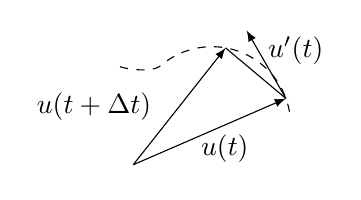
\begin{tikzpicture}
\draw[dashed]([shift={(10:1)}]1,0.5) arc (10:130:1) to [out=-135,in=180]++(-0.5,0);
\path(1,0.5)++(20:1)coordinate(kA);
\path(1,0.5)++(80:1)coordinate(kB);
\draw[-latex](0,0)--(kA)node[pos=0.6,below]{$\bM{u}(t)$};
\draw[-latex](0,0)--(kB)node[pos=0.3,above left]{$\bM{u}(t+\Delta t)$};
\draw(kA)--(kB);
\draw[-latex](kA)--++(120:1)node[pos=0.7,right]{$\bM{u}'(t)$};
\end{tikzpicture}
\caption{سمتی تفاعل کا تفرق}
\label{شکل_الاحصاء_سمتی_تفاعل_تفرق}
\end{figure}

کارتیسی نظام محدد استعمال کرتے ہوئے نقطہ \عددی{t}  پر \عددی{\bM{u}(t)} اس صورت قابل تفرق ہو گا جب اس نقطے پر درج ذیل تینوں تفرق موجود ہوں۔
\begin{align*}
u_m'(t)=\lim_{\Delta t\to 0}\frac{u_m(t+\Delta t)-u_m(t)}{\Delta t} \quad \quad (m=1,2,3)
\end{align*}
یوں سمتیہ تفاعل کا تفرق لینا اس کے تینوں ارکان کا علیحدہ علیحدہ تفرق لینے کے مترادف ہے یعنی:
\begin{align}
\bM{u}'(t)=u_1'(t)\bM{i}+u_2'(t)\bM{j}+u_3'(t)\bM{k}
\end{align}

تفرق کے جانی پہچانی اصولوں کے مطابقتی اصول سمتیہ تفاعل کے تفرق کے لئے بھی حاصل کیے جا سکتے ہیں مثلاً
\begin{align}
(c\bM{u})'=c\bM{u}' \,\, \text{(\RL{\عددی{c} مستقل ہے})},\quad \quad (\bM{u}+\bM{v})'=\bM{u}'+\bM{v}'
\end{align}
اور
\begin{align}
(\bM{u}\cdot \bM{v})'&=\bM{u}'\cdot \bM{v}+\bM{u}\cdot\bM{v}' \label{مساوات_سمتی_الاحصاء_ضرب_الف}\\
(\bM{u}\times \bM{v})'&=\bM{u}\times \bM{v}+\bM{u}\times \bM{v}'\label{مساوات_سمتی_الاحصاء_ضرب_ب}\\
\left(\frac{\bM{u}}{\bM{v}}\right)'&=\frac{\bM{v}\bM{u}-\bM{u}\bM{v}'}{\bM{v}^2}\label{مساوات_سمتی_الاحصاء_ضرب_پ}\\
(\bM{u}\bM{v}\bM{w})'&=(\bM{u}'\bM{v}\bM{w})+(\bM{u}\bM{v}'\bM{w})+(\bM{u}\bM{v}\bM{w}')\label{مساوات_سمتی_الاحصاء_ضرب_ت}
\end{align}
چونکہ سمتی ضرب غیر قابل تبادل ہے لہٰذا مساوات \حوالہ{مساوات_سمتی_الاحصاء_ضرب_ب} میں سمتیات کی ترتیب برقرار رکھنا لازم ہے۔ 

%================
\ابتدا{مثال}\quad مستقل لمبائی کے تفاعل کا تفرق\\
اگر تفاعل \عددی{\bM{u}(t)} کی لمبائی مستقل ہو یعنی \عددی{\abs{\bM{u}(t)}=c} تب  \عددی{\abs{\bM{u}}^2=\bM{u}\cdot \bM{u}=c^2} ہو گا اور مساوات \حوالہ{مساوات_سمتی_الاحصاء_ضرب_الف} کی مدد سے  \عددی{(\bM{u}\cdot \bM{u})'=2\bM{u}\cdot \bM{u}'=0} حاصل ہو گا جس کے تحت مستقل لمبائی کے سمتی تفاعل کا تفرق یا صفر سمتیہ  ہو گا اور یا یہ \عددی{\bM{u}(t)} کے قائمہ الزاویہ ہو گا۔
\انتہا{مثال}
%========================

درج بالا گفتگو سے سمتی تفاعل کی جزوی تفرق کے اصول حاصل کرتے ہیں۔اگر کسی سمتی تفاعل \عددی{\bM{u}}
\begin{align*}
\bM{u}=u_1\bM{i}+u_2\bM{j}+u_3\bM{k}
\end{align*}
کے اجزاء \عددی{n} عدد متغیرات \عددی{t_1}، \نقطے، \عددی{t_n} کے ساتھ قابل تفرق ہوں تب \عددی{t_1} کے ساتھ \عددی{\bM{u}} کے جزوی تفرق کو
 \عددی{\tfrac{\partial \bM{u}}{\partial t_1}} سے ظاہر کیا جائے گا جو درج ذیل ہو گا۔
\begin{align*}
\frac{\partial \bM{u}}{\partial t_1}=\frac{\partial u_1}{\partial t_1}\bM{i}+\frac{\partial u_2}{\partial t_1}\bM{j}+\frac{\partial u_3}{\partial t_1}\bM{k}
\end{align*}
اسی طرح دیگر جزوی تفرقات لکھے جا سکتے ہیں مثلاً:
\begin{align*}
\frac{\partial^{\,2}\bM{u}}{\partial t_m \partial t_n}=\frac{\partial^{\,2} \bM{u}_1}{\partial t_m\partial t_n}\bM{i}+\frac{\partial^{\,2} \bM{u}_2}{\partial t_m\partial t_n}\bM{j}+\frac{\partial^{\,2} \bM{u}_3}{\partial t_m\partial t_n}\bM{k}
\end{align*}

%===============
\ابتدا{مثال}\quad جزوی تفرق\\
سمتی تفاعل \عددی{\bM{r}(t_1,t_2)=a\cos \omega t_1\bM{i}+a\sin\omega t_1\bM{j}+t_2\bM{k}} کے جزوی تفرق درج ذیل ہیں۔ 
\begin{align*}
\frac{\partial \bM{r}}{\partial t_1}=a\omega (-\sin \omega t_1\bM{i}+\cos \omega t_1\bM{j}),\quad \frac{\partial \bM{r}}{\partial t_2}=\bM{k}
\end{align*}
تفاعل \عددی{\bM{r}} ایسی نلکی سطح کو ظاہر کرتا ہے جس کا رداس \عددی{a} ہے  اور محور \عددی{z} محور ہے۔ 
\انتہا{مثال}
%=================================

\حصہء{سوالات}

%==================================
سوال \حوالہ{سوال_الاحصاء_برابر_سطح_الف} تا سوال \حوالہ{سوال_الاحصاء_برابر_سطح_ب} میں برابر سطح \عددی{f=c} کیا ہو گا جہاں \عددی{c} مستقل ہے۔

%===========================
\ابتدا{سوال}\شناخت{سوال_الاحصاء_برابر_سطح_الف}\quad
$f=x+y+z$\\
جواب:متوازی سطحیں
\انتہا{سوال}
%==============================
\ابتدا{سوال}\quad
$f=x^2+y^2+z^2$\\
جواب:ہم مرکز کرہ
\انتہا{سوال}
%==============================
\ابتدا{سوال}\quad
$f=x^2+y^2$\\
جواب:کارتیسی \عددی{z}  کے ہم محوری نلکی سطحیں
\انتہا{سوال}
%==============================
\ابتدا{سوال}\quad
$f=4x^2+5y^2$\\
جواب:کارتیسی \عددی{z}  کے ہم محوری نلکی ترخیم سطحیں
\انتہا{سوال}
%==============================
\ابتدا{سوال}\شناخت{سوال_الاحصاء_برابر_سطح_ب}\quad
$f=x^2+y^2-z$\\
جواب:قطع مکافی نما سطحیں
\انتہا{سوال}
%==============================
\عددی{xy} سطح پر سمتیہ \عددی{\bM{v}} سوال \حوالہ{سوال_الاحصاء_لمبائی_سمت_الف} تا سوال \حوالہ{سوال_الاحصاء_لمبائی_سمت_ب} میں دیا گیا ہے۔وہ سطح دریافت کریں جس پر \عددی{\bM{v}} کی لمبائی مستقل ہو۔وہ سطح دریافت کریں جس پر \عددی{\bM{v}}  کی یکساں سمت ہو۔ 
%===================

\ابتدا{سوال}\شناخت{سوال_الاحصاء_لمبائی_سمت_الف}\quad 
$\bM{v}=2x\bM{i}+3y\bM{j}$\\
جوابات:
$4x^2+9y^2=\text{مستقل},\,\, \tfrac{y}{x}=\text{مستقل}$
\انتہا{سوال}
%============================
\ابتدا{سوال}\quad 
$\bM{v}=x^2\bM{i}+\sqrt{y}\bM{j}$\\
جوابات:
$x^4+y=\text{مستقل},\,\, \tfrac{\sqrt{y}}{x^2}=\text{مستقل}$
\انتہا{سوال}
%============================
\ابتدا{سوال}\quad 
$\bM{v}=(x^2-y^2)\bM{i}+2xy\bM{j}$\\
جوابات:
$x^2+y^2=\text{مستقل},\,\, \tfrac{2xy}{x^2-y^2}=\text{مستقل}$
\انتہا{سوال}
%============================
\ابتدا{سوال}\شناخت{سوال_الاحصاء_لمبائی_سمت_ب}\quad 
$\bM{v}=(x+y)\bM{i}+(x-y)\bM{j}$\\
جوابات:
$x^2+y^2=\text{مستقل},\,\, \tfrac{x-y}{x+y}=\text{مستقل}$
\انتہا{سوال}
%============================
سوال \حوالہ{سوال_الاحصاء_تفرقات_الف} تا سوال \حوالہ{سوال_الاحصاء_تفرقات_ب} میں \عددی{\bM{u}} دیا گیا ہے۔آپ سے التماس ہے کہ \عددی{\bM{u}'} اور  \عددی{\bM{u}''} دریافت کریں۔

%========================
\ابتدا{سوال}\quad \شناخت{سوال_الاحصاء_تفرقات_الف}\quad
$\bM{a}+\bM{b}t^2$\\
جوابات:
$\bM{u}'=2\bM{b}t,\,\, \bM{u}''=2\bM{b}$
\انتہا{سوال}
%============================
\ابتدا{سوال}\quad
$t\bM{i}+(t^2+2)\bM{j}$\\
جوابات:
$\bM{u}'=\bM{i}+2t\bM{j},\,\, \bM{u}''=2\bM{j}$
\انتہا{سوال}
%============================
\ابتدا{سوال}\quad
$4\cos t\,\bM{i}+2\sin t\,\bM{j}$\\
جوابات:
$\bM{u}'=-4\sin t\,\bM{i}+2\cos t\,\bM{j},\,\, \bM{u}''=-4\cos t\,\bM{i}-2\sin t\,\bM{j}=-\bM{u}$
\انتہا{سوال}
%============================
\ابتدا{سوال}\quad
$4\cos t\,\bM{i}+2\sin t\,\bM{j}-3t\,\bM{k}$\\
جوابات:
$\bM{u}'=-4\sin t\,\bM{i}+2\cos t\,\bM{j}-3\,\bM{k},\,\, \bM{u}''=-4\cos t\,\bM{i}-2\sin t\,\bM{j}$
\انتہا{سوال}
%============================
\ابتدا{سوال}\quad
$t^2\bM{i}+2 \bM{j}+4t\bM{k}$\\
جوابات:
$\bM{u}'=2t\bM{i}+4\bM{k},\,\, \bM{u}''=2\bM{i}$
\انتہا{سوال}
%============================
\ابتدا{سوال}\quad
$\cos 2t\, \bM{i}-3\sin 2t \,\bM{j}+t^2\,\bM{k}$\\
جوابات:
$\bM{u}'=-2\sin 2t\,\bM{i}-6\cos 2t\,\bM{j}+2t\,\bM{k},\,\, \bM{u}''=-4\cos 2t\,\bM{i}+12\sin 2t\,\bM{j}+2\,\bM{k}$
\انتہا{سوال}
%============================
\ابتدا{سوال}\quad
$e^{t}\, \bM{i}-2e^{-3t} \,\bM{j}$\\
جوابات:
$\bM{u}'=e^t\,\bM{i}+6e^{-3t}\,\bM{j},\,\, \bM{u}''=e^t\,\bM{i}-18e^{-3t}\,\bM{j}$
\انتہا{سوال}
%============================
\ابتدا{سوال}\quad
$e^{-t}(\cos t\, \bM{i}-\sin t \,\bM{j})$\\
جوابات:
$\bM{u}'=e^{-t}[-(\cos t+\sin t)\,\bM{i}-(\cos t-\sin t)\,\bM{j}],\,\, \bM{u}''=e^{-t}(2\sin t \,\bM{i}+2\cos t \,\bM{j})$
\انتہا{سوال}
%============================
\ابتدا{سوال}\شناخت{سوال_الاحصاء_تفرقات_ب}\quad
$t^2(2\bM{i}-5\bM{j})$\\
جوابات:
$\bM{u}'=2t(2\bM{i}-5\bM{j}),\,\, \bM{u}''=2(2\bM{i}-5\bM{j})$
\انتہا{سوال}
%============================
سوال \حوالہ{سوال_الاحصاء_ضرب_تفرق_الف} تا سوال \حوالہ{سوال_الاحصاء_ضرب_تفرق_ب} میں \عددی{\bM{u}=t\bM{i}+t^3\bM{k}}،
 \عددی{\bM{v}=t^2\bM{j}+t\bM{k}} اور \عددی{\bM{w}=2\bM{i}+t\bM{j}-t^2\bM{k}} لیتے ہوئے حل کریں۔

%===============
\ابتدا{سوال}\شناخت{سوال_الاحصاء_ضرب_تفرق_الف}\quad
$(\bM{u}\cdot \bM{v})'$\\
جواب:\عددی{4t^3}
\انتہا{سوال}
%========================
\ابتدا{سوال}\quad
$(\bM{u}\times \bM{v})'$\\
جواب:
$-t^4\bM{i}-2t\bM{j}+3t^2\bM{k}$
\انتہا{سوال}
%========================
\ابتدا{سوال}\quad
$[\bM{u}\times (\bM{v}\times \bM{w})]'$\\
جواب:
$-8t^3\bM{i}-(7t^6+5t^4-6t^2)\bM{j}+4t\bM{k}$
\انتہا{سوال}
%========================
\ابتدا{سوال}\quad
$[(\bM{u}\times \bM{v})\times \bM{w}]'$\\
جواب:
$(6t^2-7t^6)\bM{j}+(4t-6t^5)\bM{k}$
\انتہا{سوال}
%========================
\ابتدا{سوال}\شناخت{سوال_الاحصاء_ضرب_تفرق_ب}\quad
$[(\bM{u}\times \bM{v})\cdot\bM{w}]'$\\
جواب:
$-15t^4-3t^2$
\انتہا{سوال}
%========================
سوال \حوالہ{سوال_الاحصاء_جزوی_الف} تا سوال \حوالہ{سوال_الاحصاء_جزوی_ب} میں دیے گئے سمتی تفاعل \عددی{\bM{u}} کا  \عددی{x}، \عددی{y}  اور \عددی{z} کے ساتھ جزوی تفرق دریافت کریں۔

%===============
\ابتدا{سوال}\شناخت{سوال_الاحصاء_جزوی_الف}\quad
$x\bM{i}+3y\bM{k}$\\
جوابات:
$\bM{i},\,\, 3\bM{k},\,\, 0$
\انتہا{سوال}
%======================
\ابتدا{سوال}\quad
$(x^2-y^2)\bM{i}+2xy\bM{j}$\\
جوابات:
$2x\bM{i}+2y\bM{j},\,\, -2y\bM{i}+2x\bM{j},\,\, 0$
\انتہا{سوال}
%======================
\ابتدا{سوال}\quad
$x^2\bM{i}-3y^2\bM{j}+2z^2\bM{k}$\\
جوابات:
$2x\bM{i},\,\, -6y\bM{j},\,\,4z\bM{k}$
\انتہا{سوال}
%======================
\ابتدا{سوال}\quad
$xy\bM{i}+yz\bM{j}+zx\bM{k}$\\
جوابات:
$y\bM{i}+z\bM{k},\,\, x\bM{i}+z\bM{j},\,\,y\bM{j}+x\bM{k}$
\انتہا{سوال}
%======================
\ابتدا{سوال}\quad
$(x+y)\bM{i}+(y+z)\bM{j}+(z+x)\bM{k}$\\
جوابات:
$\bM{i}+\bM{k},\,\, \bM{i}+\bM{j},\,\,\bM{j}+\bM{k}$
\انتہا{سوال}
%======================
\ابتدا{سوال}\شناخت{سوال_الاحصاء_جزوی_ب}\quad
$x^2y\bM{i}+y^2z\bM{j}+z^2x\bM{k}$\\
جوابات:
$2xy\bM{i}+z^2\bM{k},\,\, x^2\bM{i}+2yz\bM{j},\,\,y^2\bM{j}+2xz\bM{k}$
\انتہا{سوال}
%======================
\ابتدا{سوال}
\عددی{(\bM{u}\cdot \bM{v})''} اور \عددی{(\bM{u}\times \bM{v})''} کے لئے مساوات \حوالہ{مساوات_سمتی_الاحصاء_ضرب_الف} اور مساوات \حوالہ{مساوات_سمتی_الاحصاء_ضرب_ب} کی طرز کے کلیات دریافت کریں۔

جوابات:
$(\bM{u}\cdot \bM{v})''=\bM{u}''\cdot \bM{v}+2\bM{u}'\cdot \bM{v}'+\bM{u}\cdot \bM{v}'' $, \\  $(\bM{u}\times \bM{v})''=\bM{u}''\times \bM{v}+2\bM{u}'\times \bM{v}'+\bM{u}\times \bM{v}''$
\انتہا{سوال}
%===========================
\ابتدا{سوال}
ثابت کریں کہ
$\left(\tfrac{\bM{u}}{\abs{\bM{u}}}\right)'=\tfrac{\bM{u}'(\bM{u}\cdot \bM{u})-\bM{u}(\bM{u}\cdot \bM{u}')}{(\bM{u}\cdot \bM{u})^{\tfrac{3}{2}}}$\\
جواب:
$\left(\tfrac{\bM{u}}{\abs{\bM{u}}}\right)'=\left(\tfrac{\bM{u}}{\sqrt{\bM{u}\cdot \bM{u}}}\right)'$
 لکھتے ہوئے  مساوات \حوالہ{مساوات_سمتی_الاحصاء_ضرب_پ} کا استعمال کریں۔
\انتہا{سوال}
%===========================

\حصہ{منحنی}
کارتیسی نظام میں منحنی \عددی{C} کو  درج ذیل سمتی تفاعل سے ظاہر کیا جا سکتا ہے (شکل \حوالہ{شکل_الاحصاء_منحنی_مقدار_معلوم}-الف)۔
\begin{align}\label{مساوات_الاحصاء_منحنی_مقدار_معلوم_الف}
\bM{r}(t)=x(t)\bM{i}+y(t)\bM{j}+z(t)\bM{k}
\end{align} 
آزاد حقیقی متغیرہ \عددی{t} کی ہر قیمت \عددی{t_0} کا \عددی{C} پر مطابقتی نقطہ پایا جاتا ہے جس  کے محدد \عددی{x(t_0)}،\عددی{y(t_0)} اور \عددی{z(t_0)} 
  تعین گر سمتیہ \عددی{\bM{r}(t_0)} دیتا ہے۔
\begin{figure}
\centering
\begin{subfigure}{0.5\textwidth}
\centering
\begin{tikzpicture}
%axis
\draw(0,0)--++(-0.25,-0.5)node[left]{$x$};
\draw(0,0)--++(1,0)node[below]{$y$};
\draw(0,0)--++(0,0.5)node[left]{$z$};
%curve
\draw(0.3,1) to [out=30,in=150]++(1.5,0.5)coordinate(kA) to [out=-30,in=-90]++(1,0.5)node[left]{$C$};
\draw[-latex](0,0)node[ocirc]{}--(kA)node[ocirc]{}node[pos=0.7,below right]{$\bM{r}(t)$};
\end{tikzpicture}
\caption*{(الف) منحنی مقدار معلوم}
\end{subfigure}%
\begin{subfigure}{0.5\textwidth}
\centering
\begin{tikzpicture}
%axis
\draw(0,0)--++(-0.25,-0.5)node[left]{$x$};
\draw(0,0)--++(1,0)node[below]{$y$};
\draw(0,0)--++(0,0.5)node[left]{$z$};
%straight line
\draw(-0.3,1)--++(2.5,0.5)node[right]{$L$}coordinate[pos=0.3](kB)coordinate[pos=0.7](kA);
\draw[-latex](0,0)node[ocirc]{}--(kA)node[ocirc]{}node[above]{$A$}node[pos=0.7,right]{$\bM{a}$};
\draw[-latex](kA)node[ocirc]{}--(kB)node[ocirc]{}node[pos=0.7,above]{$\bM{b}$};
\end{tikzpicture}
\caption*{(ب) سیدھی لکیر کا مقدار معلوم خط}
\end{subfigure}%
\caption{سیدھی لکیر اور منحنی کے مقدار معلوم خطوط۔}
\label{شکل_الاحصاء_منحنی_مقدار_معلوم}
\end{figure}
مساوات \حوالہ{مساوات_الاحصاء_منحنی_مقدار_معلوم_الف}  کو \عددی{C} کی \اصطلاح{منحنی مقدار معلوم}\فرہنگ{منحنی!مقدار معلوم}\فرہنگ{مقدار معلوم!منحنی}\حاشیہب{parametric representation}\فرہنگ{parametric!representation} کہتے ہیں جبکہ \عددی{t} کو \اصطلاح{مقدار معلوم} کہتے ہیں۔ منحنی مقدار معلوم کی طرز پر منحنی کا اظہار نہایت عمدہ ثابت ہوتا ہے۔

فضا میں منحنی ظاہر کرنے کے دیگر طریقے 
\begin{align}\label{مساوات_الاحصاء_منحنی_مقدار_معلوم_ب}
y=f(x),\quad z=g(x)
\end{align} 
اور
\begin{align}\label{مساوات_الاحصاء_منحنی_مقدار_معلوم_پ}
F(x,y,z)=0,\quad G(x,y,z)=0
\end{align}
ہیں۔مساوات \حوالہ{مساوات_الاحصاء_منحنی_مقدار_معلوم_ب} میں \عددی{x=t} پر کرتے ہوئے اس کو مساوات \حوالہ{مساوات_الاحصاء_منحنی_مقدار_معلوم_الف} کی طرح لکھ سکتے ہیں یعنی:
\begin{align*}
\bM{r}(t)=t\bM{i}+f(t)\bM{j}+g(t)\bM{k}
\end{align*}
مساوات \حوالہ{مساوات_الاحصاء_منحنی_مقدار_معلوم_پ} میں دو سطحوں کے مساوات دیے گئے ہیں جن کا ملاپ منحنی دیتا ہے۔

\اصطلاح{مستوی منحنی}\فرہنگ{مستوی!منحنی}\فرہنگ{منحنی!مستوی}\حاشیہب{plane curve}\فرہنگ{plane curve} سے مراد ایسی منحنی ہے جو فضا میں کسی سطح مستوی پر پائی جاتی ہو۔غیر مستوی منحنی کو \اصطلاح{خم دار منحنی}\فرہنگ{خم دار منحنی}\فرہنگ{منحنی!خم دار}\حاشیہب{twisted curve}\فرہنگ{twisted curve} کہتے ہیں۔

%=======================
\ابتدا{مثال}\quad سیدھا خط\\
کسی بھی سیدھی لکیر \عددی{L} کو درج ذیل لکھا جا سکتا ہے جہاں \عددی{\bM{a}} اور \عددی{\bM{b}} مستقل سمتیات ہیں (شکل \حوالہ{شکل_الاحصاء_منحنی_مقدار_معلوم}-ب)۔
\begin{align}
\bM{r}(t)=\bM{a}+t\bM{b}=(a_1+tb_1)\bM{i}+(a_2+tb_2)\bM{j}+(a_3+tb_3)\bM{k}
\end{align}
\عددی{L} نقطہ \عددی{A} سے گزرتی ہے جس کا تعین گر سمتیہ \عددی{\bM{a}} ہے جبکہ \عددی{\bM{b}} کے رخ \عددی{L}  ہو گا۔اگر \عددی{\bM{b}} اکائی سمتیہ ہو تب اس کے ارکان \اصطلاح{کوسائن رخ}\فرہنگ{کوسائن رخ}\حاشیہب{direction cosines}\فرہنگ{direction cosines} ہوں گے اور \عددی{L} پر کسی بھی نقطے کا \عددی{A} سے فاصلہ  \عددی{\abs{t}} ہو گا۔
\انتہا{مثال}
%==========================
\ابتدا{مثال}\quad ترخیم، دائرہ\\
درج ذیل سمتی تفاعل \عددی{xy} سطح میں ترخیم کو ظاہر کرتا ہے جس کا مرکز کارتیسی نظام کے مبدا  اور صدر محور \عددی{x} اور \عددی{y} محور پر ہیں۔  
\begin{align}\label{مساوات_الاحصاء_ترخیم_الف}
\bM{r}(t)=a\cos t \bM{i}+b\sin t\bM{j}
\end{align}
\عددی{x=a\cos t} اور \عددی{y=b\sin t} لیتے ہوئے \عددی{\cos^2 t+\sin^2 t=1} کے استعمال سے 
\begin{align}
\frac{x^2}{a^2}+\frac{y^2}{b^2}=1, \quad z=0
\end{align}
ملتا ہے جو ترخیم کی مساوات ہے۔اگر \عددی{a=b} ہو تب مساوات \حوالہ{مساوات_الاحصاء_ترخیم_الف} رداس \عددی{a} کی دائرے کی مساوات ہو گی۔
\انتہا{مثال}
%==============================
\ابتدا{سوال}\شناخت{مثال_الاحصاء_پیچ_دار}\quad پیچ دار لچھا\\
\اصطلاح{پیچ دار لچھے}\فرہنگ{پیچ دار لچھا}\حاشیہب{circular helix}\فرہنگ{helix!circular} کو
\begin{align}
\bM{r}(t)=a\cos t\bM{i}+a\sin t\bM{j}+ct\bM{k}\quad \quad (c \ne 0)
\end{align}
ظاہر کرتا ہے۔اس \اصطلاح{خم دار منحنی} کو \عددی{c>0} (دایاں ہاتھ پیچ دار لچھا) اور \عددی{c<0} (بایاں ہاتھ پیچ دار لچھا) کے لئے  شکل \حوالہ{شکل_الاحصاء_پیچدار} میں دکھایا گیا ہے۔
\begin{figure}
\centering
\begin{subfigure}{0.5\textwidth}
\centering
\begin{tikzpicture}[x={(-0.5cm,-0.5cm)},y={(1cm,0cm)},z={(0cm,1cm)}]
\pgfmathsetmacro{\ang}{30}
\pgfmathsetmacro{\h}{1.5}
\pgfmathsetmacro{\c}{\h/450}
%axis
\draw(0.075,0,0)--(1.5,0,0)node[left]{$x$};
\draw(0,0.075,0)--(0,1.5,0)node[below]{$y$};
\draw[dashed](0,0,0)--(0,0,\h);
\draw(0,0,\h)--++(0,0,1)node[left]{$z$};
%curve
\draw[domain=0:90+\ang,smooth,variable=\t] plot ({cos(\t)},{sin(\t)},{\c*\t});
\draw[dashed,domain=90+\ang:270+\ang,smooth,variable=\t] plot ({cos(\t)},{sin(\t)},{\c*\t});
\draw[domain=270+\ang:450,smooth,variable=\t] plot ({cos(\t)},{sin(\t)},{\c*\t});
%arrow
\draw[-stealth] ({cos(80)},{sin(80)},{\c*80})--({cos(82)},{sin(82)},{\c*82});
%cylinder
\draw[domain=-90+\ang:90+\ang,smooth,variable=\t] plot ({cos(\t)},{sin(\t)},{0})coordinate(kA);
\draw(kA)--++(0,0,\h);
\draw({cos(-90+\ang)},{sin(-90+\ang)},0)--++(0,0,\h);
\draw[domain=0:360,smooth,variable=\t] plot ({cos(\t)},{sin(\t)},{\h})coordinate(kA);
%nodes
\draw[domain=-130:150,smooth,variable=\t] plot ({0.075*cos(\t)},{0.075*sin(\t)},{\h});
\path (1,0,0)node[ocirc]{};
\path[domain=270+\ang:450,smooth,variable=\t] plot ({cos(\t)},{sin(\t)},{\c*\t})node[ocirc]{};
\draw[domain=-130:150,smooth,variable=\t] plot ({0.075*cos(\t)},{0.075*sin(\t)},{0});
\end{tikzpicture}
\caption*{(الف) دایاں ہاتھ پیچ دار لچھا}
\end{subfigure}%
\begin{subfigure}{0.5\textwidth}
\centering
\begin{tikzpicture}[x={(-0.5cm,-0.5cm)},y={(1cm,0cm)},z={(0cm,1cm)}]
\pgfmathsetmacro{\ang}{30}
\pgfmathsetmacro{\h}{-1.5}
\pgfmathsetmacro{\c}{\h/450}
%axis
\draw(0.075,0,0)--(3,0,0)node[left]{$x$};
\draw(0,0.075,0)--(0,2,0)node[below]{$y$};
\draw(0,0,0)--(0,0,1)node[left]{$z$};
%curve
\draw[domain=0:90+\ang,smooth,variable=\t] plot ({cos(\t)},{sin(\t)},{\c*\t});
\draw[dashed,domain=90+\ang:270+\ang,smooth,variable=\t] plot ({cos(\t)},{sin(\t)},{\c*\t});
\draw[domain=270+\ang:450,smooth,variable=\t] plot ({cos(\t)},{sin(\t)},{\c*\t});
%arrow
\draw[-stealth] ({cos(80)},{sin(80)},{\c*80})--({cos(82)},{sin(82)},{\c*82});
%cylinder
\draw[domain=-90+\ang:90+\ang,smooth,variable=\t] plot ({cos(\t)},{sin(\t)},{\h})coordinate(kA);
\draw(kA)--++(0,0,-\h);
\draw({cos(-90+\ang)},{sin(-90+\ang)},0)--++(0,0,\h);
\draw[domain=0:360,smooth,variable=\t] plot ({cos(\t)},{sin(\t)},{0})coordinate(kA);
%nodes
\path (1,0,0)node[ocirc]{};
\path[domain=270+\ang:450,smooth,variable=\t] plot ({cos(\t)},{sin(\t)},{\c*\t})node[ocirc]{};
\draw[domain=-130:150,smooth,variable=\t] plot ({0.075*cos(\t)},{0.075*sin(\t)},{0});
\end{tikzpicture}
\caption*{(ب) بایاں ہاتھ پیچ دار لچھا}
\end{subfigure}%
\caption{پیچ دار لچھے (مثال \حوالہ{مثال_الاحصاء_پیچ_دار})۔}
\label{شکل_الاحصاء_پیچدار}
\end{figure}
\انتہا{سوال}
%====================================

ہم قطع منحنی اپنی آپ کو قطع کرتی ہے۔ نقطہ قطع کو منحنی کا \اصطلاح{متعدد نقطہ}\فرہنگ{متعدد نقطہ}\حاشیہب{multiple point}\فرہنگ{multiple point} کہتے ہیں (شکل \حوالہ{شکل_الاحصاء_دوہرا_نقطہ})۔ ایسی منحنی جس کے متعدد نقطے نہ پائے جاتے ہوں \اصطلاح{سادہ منحنی}\فرہنگ{سادہ منحنی}\فرہنگ{منحنی!سادہ}\حاشیہب{simple curve}\فرہنگ{curve!simple} کہلاتی ہے۔
\begin{figure}
\centering
\begin{subfigure}{0.5\textwidth}
\centering
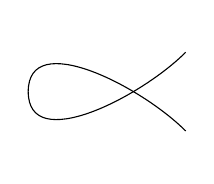
\begin{tikzpicture}
\draw(0,0) to [out=90,in=135]++(2,-0.5);
\draw(0,0) to [out=-90,in=-135]++(2,0.5);
\end{tikzpicture}
\end{subfigure}%
\begin{subfigure}{0.5\textwidth}
\centering
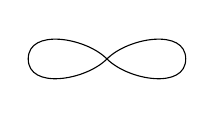
\begin{tikzpicture}
\draw(0,0) to [out=90,in=135]++(1,0) to [out=-45,in=-90]++(1,0);
\draw(0,0) to [out=-90,in=-135]++(1,0) to [out=45,in=90]++(1,0);
\end{tikzpicture}
\end{subfigure}%
\caption{دوہرا نقطوں والے منحنی}
\label{شکل_الاحصاء_دوہرا_نقطہ}
\end{figure}

%===============
\ابتدا{مثال}\quad سادہ اور غیر سادہ منحنی\\
ترخیم اور پیچ دار لچھے سادہ ترخیم کی مثالیں ہیں۔درج ذیل \عددی{t=1} اور \عددی{t=-1} پر مبدا سے دو مرتبہ گزرتی ہے لہٰذا یہ غیر سادہ منحنی کی مثال ہے۔
\begin{align*}
\bM{r}(t)=(t^2-1)\bM{i}+(t^3-1)\bM{j}
\end{align*}
\انتہا{مثال}
%=========================

آخر میں بتاتا چلوں کہ کسی بھی منحنی \عددی{C} کو کئی سمتی تفاعل سے ظاہر کیا جا سکتا ہے مثلاً اگر \عددی{C} کو مساوات \حوالہ{مساوات_الاحصاء_منحنی_مقدار_معلوم_الف} ظاہر کرے تب ہم \عددی{t=h(t^*)} لیتے ہوئے، جہاں مساوات \حوالہ{مساوات_الاحصاء_منحنی_مقدار_معلوم_الف} میں استعمال \عددی{t} کی تمام قیمتوں کے لئے  \عددی{h(t^*)} بھی پائے جاتے ہوں،  \عددی{C} کو نئی سمتی تفاعل \عددی{\tilde{\bM{r}}(t^*)=\bM{r}[h(t^*)]} سے ظاہر کر سکتے ہیں۔

%============
\ابتدا{مثال}\quad مقدار معلوم کی تبدیلی\\
\عددی{xy} سطح میں قطع مکافی \عددی{y=x^2} کو درج ذیل سمتیہ تفاعل ظاہر کرتی ہے۔
\begin{align}
\bM{r}=t\bM{i}+t^2\bM{j}\quad \quad (-\infty < t < \infty)
\end{align}
ہم \عددی{t=-2t^*} لیتے ہوئے اس قطع مکافی کو درج ذیل سمتی تفاعل سے ظاہر کر سکتے ہیں۔
\begin{align*}
\tilde{\bM{r}}(t^*)=\bM{r}(-2t^*)=-2t^*\bM{i}+4t^{*2}\bM{j}
\end{align*}
اگر ہم \عددی{t=t^{*2}} لیں تب ہمیں درج ذیل نیا سمتی تفاعل ملتا ہے
\begin{align*}
\tilde{\bM{r}}(t^*)=t^{*2}\bM{i}+t^{*4}\bM{j}
\end{align*} 
لیکن \عددی{t^{*2}>0} کی بنا یہ تفاعل قطع مکافی کو صرف ربع اول میں ظاہر کرتا ہے۔
\انتہا{مثال}
%======================

\حصہء{سوالات}
سوال \حوالہ{سوال_الاحصاء_مقدار_معلوم_خط_الف} تا سوال \حوالہ{سوال_الاحصاء_مقدار_معلوم_خط_ب} میں نقطہ \عددی{A} سے گزرتی ہوئی سمتیہ \عددی{\bM{b}} کے رخ سیدھی لکیر کی مقدار معلوم مساوات دریافت کریں۔

%================
\ابتدا{سوال}\شناخت{سوال_الاحصاء_مقدار_معلوم_خط_الف}\quad 
$A:(0,0,0),\quad \bM{b}=\bM{i}-\bM{j}$\\
جواب:
$\bM{r}=t\bM{i}-t\bM{j}$
\انتہا{سوال}
%====================
\ابتدا{سوال}\quad 
$A:(2,-3,1),\quad \bM{b}=\bM{i}+2\bM{j}$\\
جواب:
$\bM{r}=(t+2)\bM{i}+(2t-3)\bM{j}+\bM{k}$
\انتہا{سوال}
%====================
\ابتدا{سوال}\quad 
$A:(2,0,-3),\quad \bM{b}=-\bM{j}+3\bM{k}$\\
جواب:
$\bM{r}=2\bM{i}-t\bM{j}+3(t-1)\bM{k}$
\انتہا{سوال}
%====================
\ابتدا{سوال}\شناخت{سوال_الاحصاء_مقدار_معلوم_خط_ب}\quad 
$A:(-3,2,6),\quad \bM{b}=5\bM{i}+3\bM{j}-7\bM{k}$\\
جواب:
$\bM{r}=(5t-3)\bM{i}+(3t+2)\bM{j}+(6-7t)\bM{k}$
\انتہا{سوال}
%====================
سوال \حوالہ{سوال_الاحصاء_مقدار_معلوم_سیدھی_لکیر_الف} تا سوال \حوالہ{سوال_الاحصاء_مقدار_معلوم_سیدھی_لکیر_ب} میں نقطہ \عددی{A} اور نقطہ \عددی{B} سے گزرتی ہوئی سیدھی لکیر کی مقدار معلوم مساوات دریافت کریں۔

%=========
\ابتدا{سوال}\شناخت{سوال_الاحصاء_مقدار_معلوم_سیدھی_لکیر_الف} \quad
$A:(0,0,0),\quad B:(1,1,1)$\\
جواب:
$\bM{r}=t\bM{i}+t\bM{j}+t\bM{k}$
\انتہا{سوال}
%======================
\ابتدا{سوال}\quad
$A:(-3,7,-5),\quad B:(2,0,3)$\\
جواب:
$\bM{r}=(5t-3)\bM{i}+7(1-t)\bM{j}+(8t-5)\bM{k}$
\انتہا{سوال}
%======================
\ابتدا{سوال}\quad
$A:(1,2,-3),\quad B:(7,2,-3)$\\
جواب:
$\bM{r}=(6t+1)\bM{i}+2\bM{j}-3\bM{k}$
\انتہا{سوال}
%======================
\ابتدا{سوال}\شناخت{سوال_الاحصاء_مقدار_معلوم_سیدھی_لکیر_ب}\quad
$A:(3,2,0),\quad B:(0,0,0)$\\
جواب:
$\bM{r}=3(1-t)\bM{i}+2(1-t)\bM{j}$
 جس میں \عددی{t^*=1-t} چنتے ہوئے 
$\tilde{\bM{r}}=3t^*\bM{i}+2t^*\bM{j}$
 بھی لکھا جا سکتا ہے۔
\انتہا{سوال}
%======================

سوال \حوالہ{سوال_الاحصاء_مقدار_معلوم_درکار_الف} تا سوال \حوالہ{سوال_الاحصاء_مقدار_معلوم_درکار_ب} میں دیے سیدھی لکیر کی مقدار معلوم مساوات دریافت کریں۔

%==============
\ابتدا{سوال}\شناخت{سوال_الاحصاء_مقدار_معلوم_درکار_الف}\quad
$y=x,\quad z=0$\\
جواب:
$\bM{r}=t\bM{i}+t\bM{j}$
\انتہا{سوال}
%=====================
\ابتدا{سوال}\quad
$y=-3x,\quad z=2x$\\
جواب:
$\bM{r}=t\bM{i}-3t\bM{j}+2t\bM{k}$
\انتہا{سوال}
%=====================
\ابتدا{سوال}\quad
$2y=5x,\quad z=x-3y$\\
جواب:
$\bM{r}=t\bM{i}+\tfrac{5}{2}\bM{j}-\tfrac{13}{2}\bM{k}$ \quad 
یا \quad 
$\bM{r}=2t\bM{i}+5t\bM{j}-13t\bM{k}$\quad 
جہاں \عددی{t^*} کی جگہ \عددی{t} ہی لکھا گیا ہے۔
\انتہا{سوال}
%=====================
\ابتدا{سوال}\quad
$4x-y+z=3,\quad -3x+2y+3z=19$\\
جواب:\عددی{y} اور \عددی{z} حاصل کرتے ہوئے  \quad
$\bM{r}=t\bM{i}+(3t+2)\bM{j}+(5-t)\bM{k}$
\انتہا{سوال}
%=====================
\ابتدا{سوال}\شناخت{سوال_الاحصاء_مقدار_معلوم_درکار_ب}\quad
$x-y=2,\quad 2x+z=3$\\
جواب:
$\bM{r}=t\bM{i}+(t-2)\bM{j}+(3-2t)\bM{k}$
\انتہا{سوال}
%=====================
سوال \حوالہ{سوال_الاحصاء_عمومی_مقدار_معلوم_الف} تا سوال \حوالہ{سوال_الاحصاء_عمومی_مقدار_معلوم_ب} میں دیے خطوط کی مقدار معلوم مساوات دریافت کریں۔

%================
\ابتدا{سوال}\شناخت{سوال_الاحصاء_عمومی_مقدار_معلوم_الف} \quad
$x^2+y^2=1,\quad z=0$\\
جواب:
$\bM{r}=\cos t\bM{i}+\sin t\bM{j}$
\انتہا{سوال}
%===================
\ابتدا{سوال}\quad
$y=x^3,\quad z=0$\\
جواب:
$\bM{r}=t\bM{i}+t^3\bM{j}$
\انتہا{سوال}
%===================
\ابتدا{سوال}\quad
$y=2x^3,\quad z=-3x^2$\\
جواب:
$\bM{r}=t\bM{i}+2t^3\bM{j}-3t^2\bM{k}$
\انتہا{سوال}
%===================
\ابتدا{سوال}\quad
$x^2+y^2-4x+6y=-9,\quad z=0$\\
جواب: نقطہ \عددی{(2,-3)} پر رداس \عددی{2} کا دائرہ \quad
$\bM{r}=(2+2\cos t)\bM{i}+(-3+2\sin t)\bM{j}$
\انتہا{سوال}
%===================
\ابتدا{سوال}\quad
$4(x+1)^2+y^2=4,\quad z=0$\\
جواب:
$\bM{r}=(-1+2\cos t)\bM{i}+2\sin t\bM{j}$
\انتہا{سوال}
%===================
\ابتدا{سوال}\شناخت{سوال_الاحصاء_عمومی_مقدار_معلوم_ب}\quad
$x^2+y^2=4,\quad z=e^{-x}$\\
جواب:
$\bM{r}=2\cos t\bM{i}+2\sin t\bM{j}+e^{-t}\bM{k}$
\انتہا{سوال}
%===================
